\section{Pernyataan Tidak Melakukan Kecurangan}
Tugas ini disusun sepenuhnya tanpa bantuan kecerdasan buatan (Generative AI), melainkan hasil pemikiran dan analisis mandiri.
\begin{center}
    \begin{minipage}{\dimexpr\linewidth-2\fboxsep-2\fboxrule\relax}
        \hfill
        \begin{minipage}[t]{0.28\linewidth}\centering
            \vspace{-2pt}% adjust top alignment
            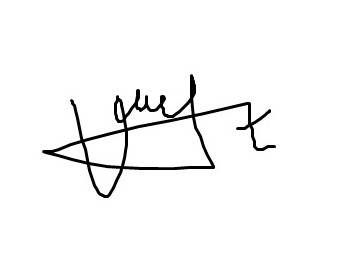
\includegraphics[width=3cm]{public/ttd-vincent.jpeg}\\[4pt]
            Vincent Rionarlie\\
            13524031\\[12pt]

            
\includegraphics[width=3cm]{public/ttd-jason.png}\\[4pt]
            Jason Edward Salim\\
            13524034\\[12pt]

            
\includegraphics[width=3cm]{public/ttd-aufar.png}\\[4pt]
            Muhammad Aufar Rizqi Kusuam\\
            13524061
        \end{minipage}
    \end{minipage}%
\end{center}


\section{Tautan GitHub}
\href{https://github.com/Vixrlie/Tubes3_SL0T999}{Link GitHub}

\section{Tabel Checklist Spesifikasi}
\begin{center}
    \rowcolors{2}{gray!15}{white}
    \begin{tabularx}{\linewidth}{C{0.7cm} X C{1.0cm} C{1.0cm}}
        \toprule
        \textbf{No} & \textbf{Poin}                                                                                                                    & \textbf{Ya} & \textbf{Tidak} \\
        \midrule
        1           & Extension berhasil di-build dan di-load tanpa kesalahan pada Chromium browser dan dikembangkan dengan TypeScript                 &             &                \\
        2           & KMP dan Boyer-Moore diimplementasikan from scratch                                                                               &             &                \\
        3           & Regex meng-handle format \textless kata\textgreater\textless angka\textgreater dan berbagai edge case                            &             &                \\
        4           & Pencarian KMP \& BM membaca `keywords.txt` secara iteratif dan tidak menggunakan built-in search function atau library eksternal &             &                \\
        5           & Exact matching dan fuzzy matching berjalan benar                                                                                 &             &                \\
        6           & Elemen DOM terdeteksi diberi highlight dan terhapus saat rescanning                                                              &             &                \\
        7           & Tooltip muncul saat hover dengan informasi keyword, algoritma, kemunculan, dan waktu eksekusi                                    &             &                \\
        8           & Popup menampilkan statistik realtime (total keyword, perbandingan, waktu eksekusi, jumlah match)                                 &             &                \\
        9           & [Bonus] Membuat Video YouTube (jika dikerjakan)                                                                                  &             &                \\
        10          & [Bonus] Implementasi Algoritma Aho-Corasick dan Rabin-Karp                                                                       &             &                \\
        11          & [Bonus] Implementasi Censorship / Blur Teks dengan toggle on/off                                                                 &             &                \\
        12          & [Bonus] Implementasi Optical Character Recognition pada Gambar                                                                   &             &                \\
        \bottomrule
    \end{tabularx}
\end{center}

\section{Tabel Kontribusi}
\begin{center}
    \rowcolors{2}{gray!15}{white}
    \begin{tabularx}{\linewidth}{C{0.8cm} Y C{2.8cm} Y C{2.2cm}}
        \toprule
        \textbf{No} & \textbf{Nama Lengkap}       & \textbf{NIM} & \textbf{Deskripsi Pekerjaan}                                                                      & \textbf{Persentase Kontribusi (\%)} \\
        \midrule
        1           & Vincent Rionarlie           & 13524031     & Pembuatan algoritma pemrosesan string, bonus algortima Aho-Corasick dan Rabin-Karp, laporan akhir & 34                                  \\
        2           & Jason Edward Salim          & 13524034     & Pembuatan FE beserta dengan build-up nya, bonus censoring, laporan akhir                          & 33                                  \\
        3           & Muhammad Aufar Rizqi Kusuam & 13524061     & Pembuatan Controller program (Scanner, highlighter, DOM Integration, dll), laporan akhir          & 33                                  \\
        \bottomrule
    \end{tabularx}
\end{center}

% Isi kolom "Deskripsi Pekerjaan" dan persentase sesuai pembagian kerja sebenarnya.